 \documentclass[a4paper,twoside,10pt]{report}
%% ___Ent�te pour mouline.sh________________________
% Usage : ./mouline.sh dvi moncul  (pour moncul.tex)
%         ./mouline.sh pdf moncul
%    reverse search en dvi avec CTRL+click

\pdfoutput=1

\usepackage{graphicx}

\ifnum\pdfoutput<1 \DeclareGraphicsExtensions{.eps}
\newcommand{\inputxfig}[1]{\includegraphics{#1.eps}}
\usepackage[hypertex]{hyperref} 
\else
\DeclareGraphicsExtensions{.pdf}
\newcommand{\inputxfig}[1]{\input{#1.pdftex_t}}
\usepackage[pdftex,hypertexnames=false]{hyperref} \fi
%% ____Chemin pour les figures pour mouline.sh_______

\graphicspath{{figures/}}
%% __________________________________________________


%% ________________extensions________________________
\usepackage[T1]{fontenc} 
\usepackage[latin1]{inputenc}
\usepackage{latexsym} 
\usepackage{ae} 
\usepackage{aecompl}
\usepackage[cyr]{aeguill}

\usepackage[french]{babel}             % distribution french 
\usepackage[french]{varioref}

\usepackage{caption}
\usepackage{float}
\usepackage{color}%\usepackage{lscape}
%\usepackage{longtable}
%\usepackage{amsthm,amssymb,amsmath,amsfonts}

% pour les tableaux
\usepackage{multicol}
\usepackage{multirow}


%%_______________environnements maison______________

\def\stackunder#1#2{
  \mathrel{\mathop{#2}\limits_{#1}}
}
\newtheorem{theo}{Th�or�me}
\newcommand{\normalsubformula}[1]{#1}
\newcommand{\vectD}[2]{
  \begin{array}[l]{l}
    #1\\
    #2
  \end{array}
}
\newcommand{\matNM}[2]{
  \begin{array}[l]{l}
    {}_{_{\underline{{#2}}}}\\
    \Box|_{_{#1}}
  \end{array}  
}

% *************** les nouvelles commandes ***************

\definecolor{gris}{gray}{0.50}
\newcommand{\important}[1]{
  \petitSaut \begin{tabular}{|p{0.9\linewidth}|}
    \hline 
    #1\\
    \hline
  \end{tabular} \petitSaut
}

% indentation multiple
\newcommand{\dindent}{\indent \indent }
\newcommand{\tindent}{\indent \indent \indent}
\newcommand{\qindent}{\dindent \dindent }
\newcommand{\cindent}{\dindent \dindent \indent}

\newcommand{\sautLigne}{\vspace{0.7cm}}
\newcommand{\petitSaut}{\vspace{0.2cm}}



\hyphenation{nom-bre} 




%%___________________MISE EN PAGE____________________
%\setlength{\hoffset}{1cm}
%\setlength{\textwidth}{16cm}
\addtolength{\textwidth}{6cm}
%\setlength{\oddsidemargin}{0cm}
%\setlength{\evensidemargin}{0cm}
\setlength\oddsidemargin{-0.5cm}
\setlength\evensidemargin{-1.5cm}
%\addtolength\marginparwidth{0.5cm}
\addtolength\topmargin{-1.5cm}
\addtolength\textheight{3cm}
\addtolength\columnsep{0.5cm}

%%___Style et pieds de pages___________________
\newcommand{\piedbasgauche}{BE m�tro (Autom \& CAN \& TR)}
\newcommand{\piedbasdroit}{5 TRS}

%%______Style du poly________________________________
%
\newfont{\scaledfont}{cmr12 scaled 4000}
\renewcommand{\thechapter}{\arabic{chapter}}
\makeatletter
\def\@makechapterhead#1{
  {\parindent \z@ \raggedright \normalfont
    \interlinepenalty\@M
    \parbox{0.70\textwidth}{\Huge \bfseries #1}\ %
    \hfill\scaledfont{\thechapter}\par\normalsize%
    \rule{\textwidth}{1pt}%  <--- the rule
    \nobreak
    \vskip 40\p@
  }%
}
\makeatother


%%________renomme les chapitres _________
\addto\captionsfrench{%
\renewcommand{\chaptername}{Chapitre}
%\renewcommand{\chaptermark}[1]{\markboth{\chaptername~\thechapter~:#1}{}} %
}


%%______entête et pieds de page géniaux________

\usepackage{fancyhdr}
\pagestyle{fancy}


\addtolength{\headheight}{0.2\baselineskip} % Pour éviter le overfull \vbox .... has occured while ouput  is active voir doc fancyhdr

\addtolength{\parskip}{0.4\baselineskip}

%%%%%%%%%%%%%%%%%
%% PAGES DE GAUCHE (PAGES PAIRES) Cas de deux faces
%%%%%%%%%%%%%%
\fancyhead[LE]{\thepage}                                        % Indications en haut à gauche
\fancyhead[CE]{}                                                % Indications en haut au centre
\fancyhead[RE]{\leftmark}                                       % Indications en haut à droite
\fancyfoot[LE]{\tiny \piedbasgauche{}}     % Indications en bas à gauche
\fancyfoot[CE]{}                                                % Indications en bas au centre
\fancyfoot[RE]{}                                                % Indications en bas à doite
%%%%%%%%%%%%%%%%%
%% PAGES DE DROITE (PAGES IMPAIRES) Cas de deux faces
%%%%%%%%%%%%%%
\fancyhead[LO]{\rightmark}                                      % Indications en haut à gauche
\fancyhead[CO]{}                                                % Indications en haut au centre
\fancyhead[RO]{\thepage}                                        % Indications en haut à droite
\fancyfoot[LO]{}                                                % Indications en bas à gauche
\fancyfoot[CO]{}                                                % Indications en bas au centre
\fancyfoot[RO]{\tiny \piedbasdroit{}}     % Indications en bas à doite


%%%%%%%%%%%%%%%%%
%% PAGES DE GAUCHE (PAGES PAIRES) Cas de une face
%%%%%%%%%%%%%%
%\fancyhead[LE]{}    % Indications en haut à gauche
%\fancyhead[CE]{}   % Indications en haut au centre
%\fancyhead[RE]{}    % Indications en haut à droite
%\fancyfoot[LE]{}     % Indications en bas à gauche
%\fancyfoot[CE]{}    % Indications en bas au centre
%\fancyfoot[RE]{}      % Indications en bas à doite
%%%%%%%%%%%%%%%%%
%% PAGES DE DROITE (PAGES IMPAIRES) Cas de une face
%%%%%%%%%%%%%%
%\fancyhead[LO]{\rightmark}    % Indications en haut à gauche
%\fancyhead[CO]{}   % Indications en haut au centre
%\fancyhead[RO]{\thepage}    % Indications en haut à droite
%\fancyfoot[LO]{\leftmark}     % Indications en bas à gauche
%\fancyfoot[CO]{}    % Indications en bas au centre
%\fancyfoot[RO]{\tiny Sébastien \textsc{Bosch} - LAAS-RIA -
%\today}


\renewcommand{\headrulewidth}{0.4pt}
%\renewcommand{\footrulewidth}{0.4pt}



\begin{document}

	\thispagestyle{empty}
	
	\begin{center}
	
	  \begin{tabular}[l]{ll}
	    
\includegraphics[width=3cm]{logo_insa}\hspace{0.5cm}
	
	    &\vspace{-1.3cm} \\
	
	    &\textsc{Minist�re  de l'Emmerdement Sup�rieur et du temps qui passe}\\
	    &\vspace{0cm}\textsc{D�partement du G�nie �lectrique et Informatique}
	
	  \end{tabular}
	
	\end{center}
	
	\vspace{1.5cm}
	
	\begin{center}
	  {\LARGE \textsc{Bureau d'�tude Syst�mes Embarqu�s Distribu�s}} 
	
	\vspace{1cm}
	
	
	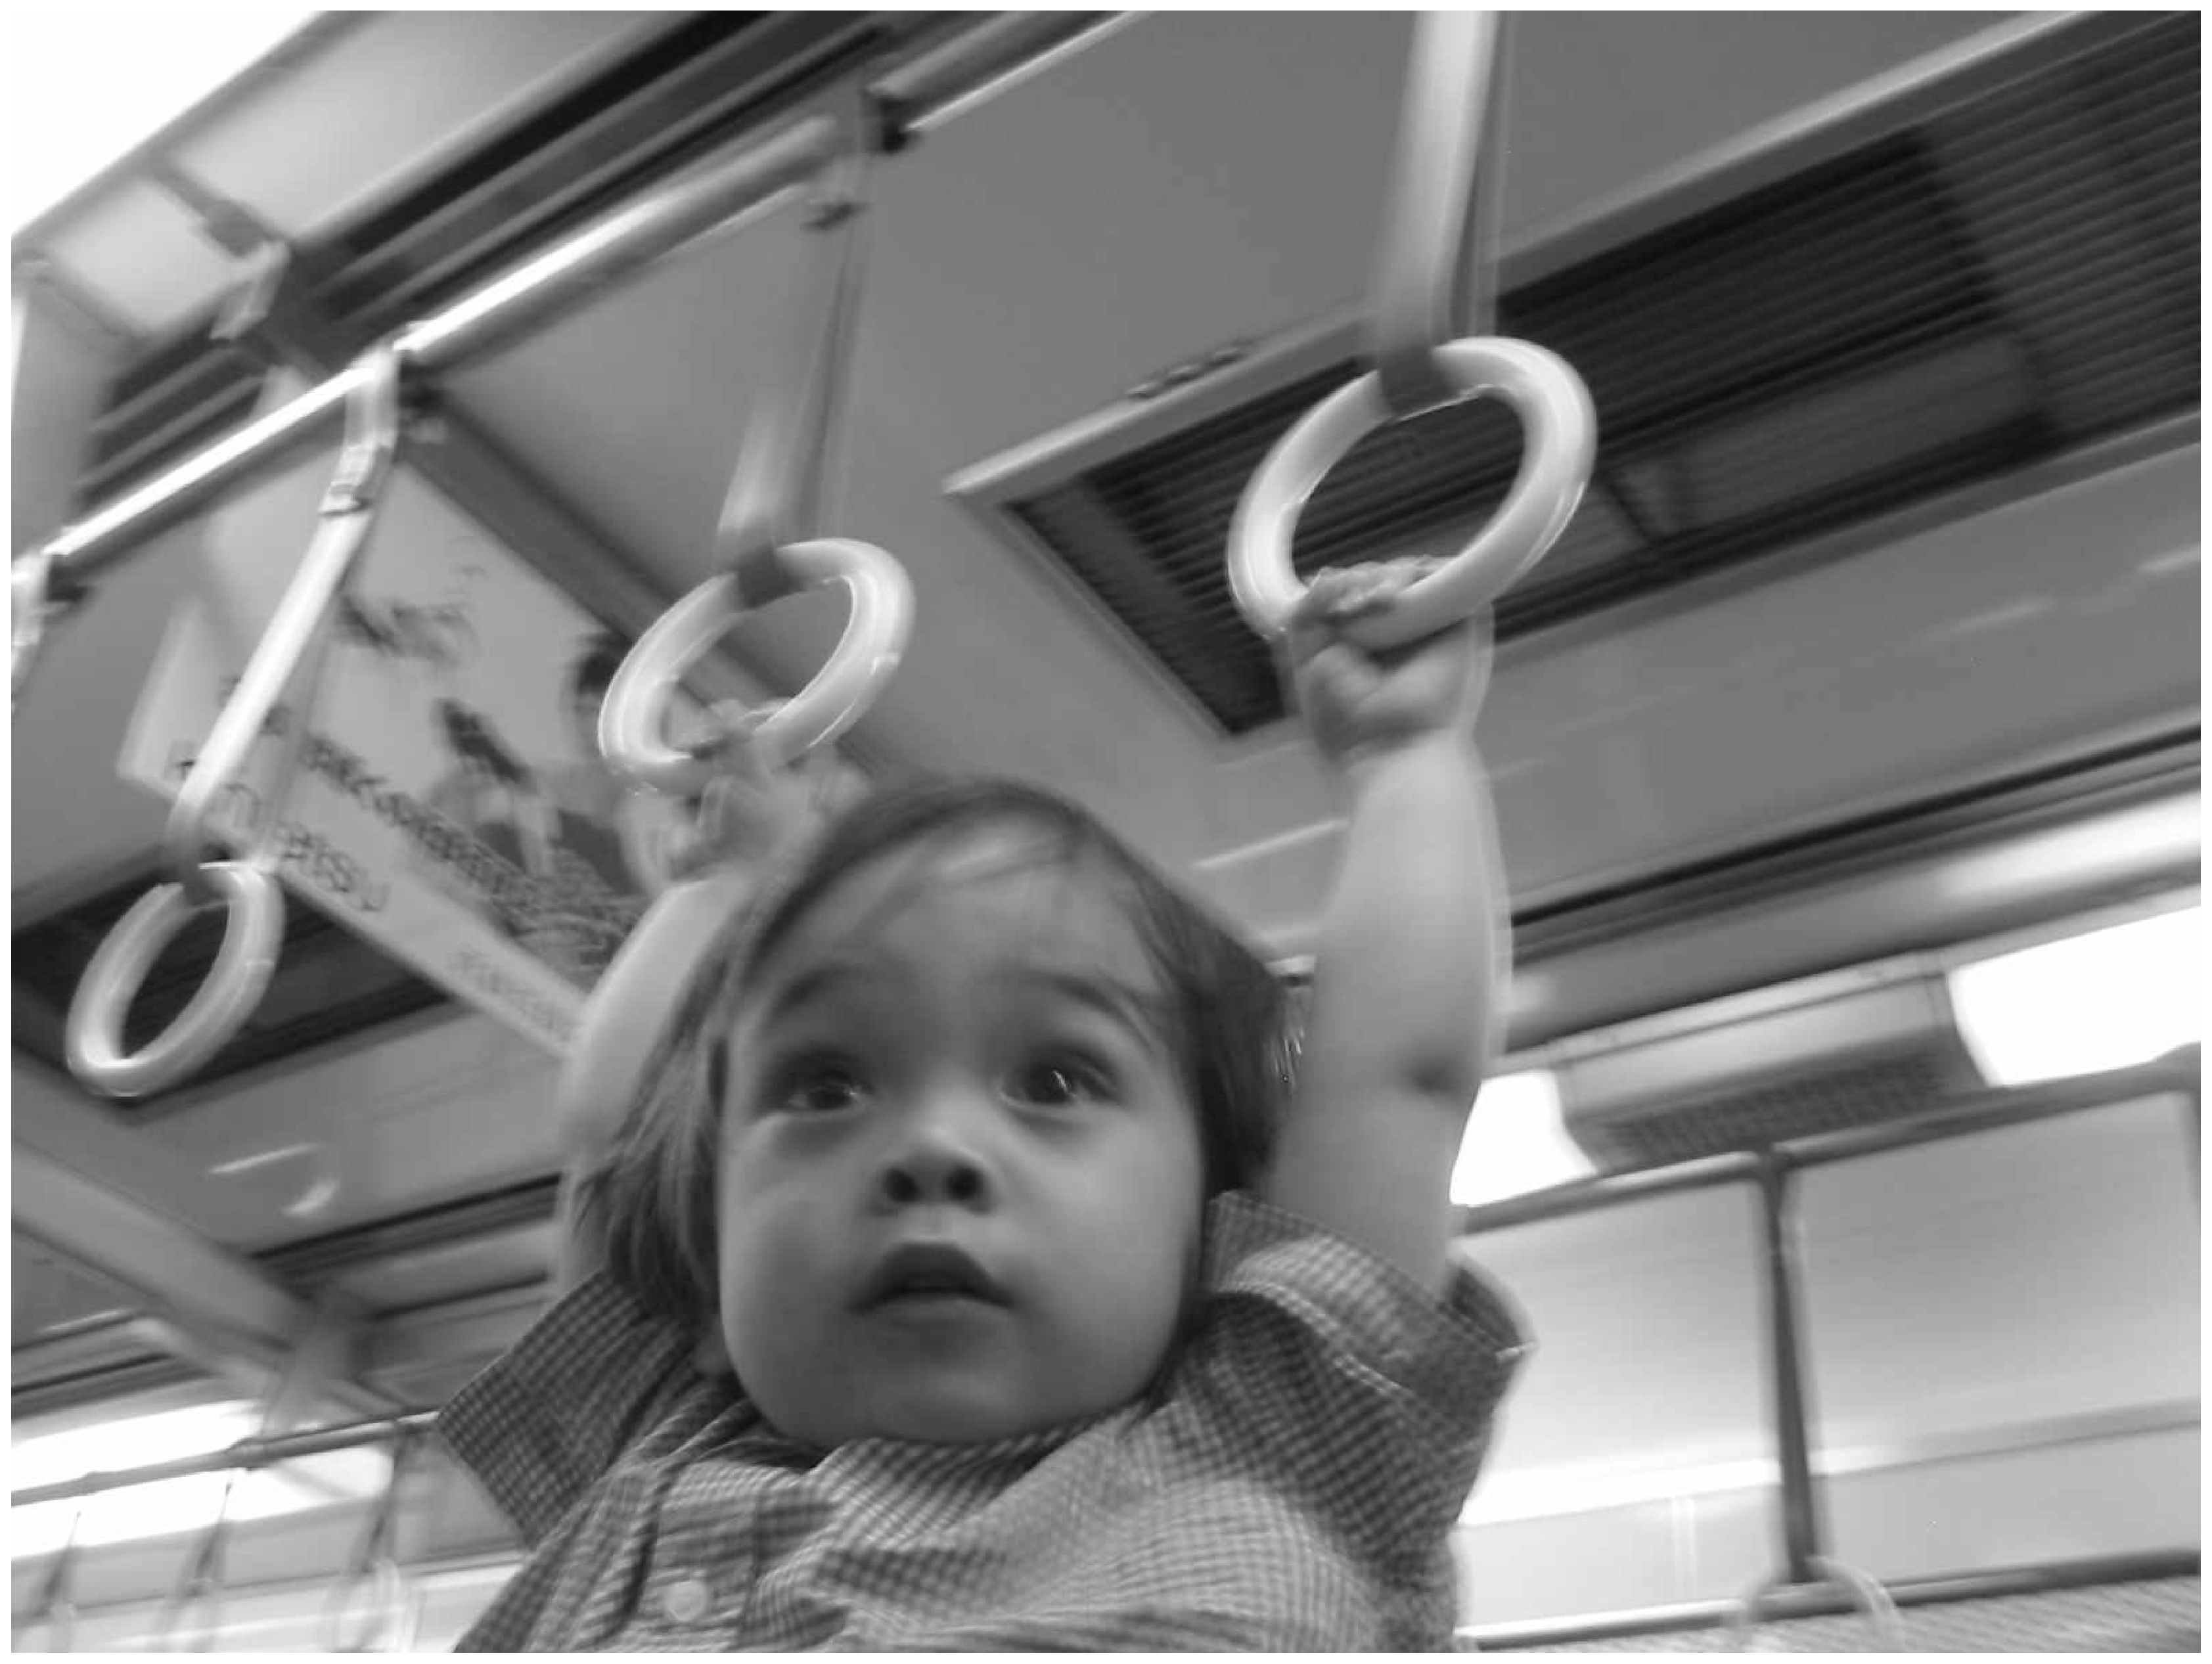
\includegraphics[width=0.9\textwidth]{kyle_on_subway}
	
	\vspace{2cm}
	
	{\Large M�tropolitain}
	  
	\vspace{2cm}
	
	
	 
	\end{center}
	
	\begin{tabular}[c]{l}
	{\large version 2009--2010}  \\
    \end{tabular}


\cleardoublepage

\chapter{Pr�sentation du BE}

On veut concevoir une rame de m�tro r�volutionnaire puisque
les voitures ne seraient pas li�es m�caniquement
entre--elles~! Les avantages sont multiples : la r�duction
du co�t de fabrication, la flexibilit� d'utilisation lors de
l'ajout de voitures � la rame.

On envisage que chaque voiture poss�de son propre
calculateur reli� aux autres par un bus CAN (passant par les
rails) permettant d'�changer les informations entre voitures
afin d'�viter toute collision.

Il s'agit alors de commander le moteur de chaque voiture
de mani�re � �viter les collisions et � poursuivre une
trajectoire permettant de relier les diff�rentes stations
dans les temps impartis. 

Votre BE consiste � r�aliser les logiciels embarqu�s sur un
prototype miniature de la future rame. Dans ce prototype les
voitures sont mat�rialis�es par des mod�le r�duits sur-�quip�s par nos soins. 
Le bus CAN est filaire et les calculateurs
sont de redoutables STM32F103RB (coeur Cortex-M3).


La fig.~\ref{FigUseCase} repr�sente le diagramme
d'utilisation des diff�rentes entit�s logicielles.
\begin{figure}[h!tbp]
  \begin{center}
    \resizebox{0.9\linewidth}{!}{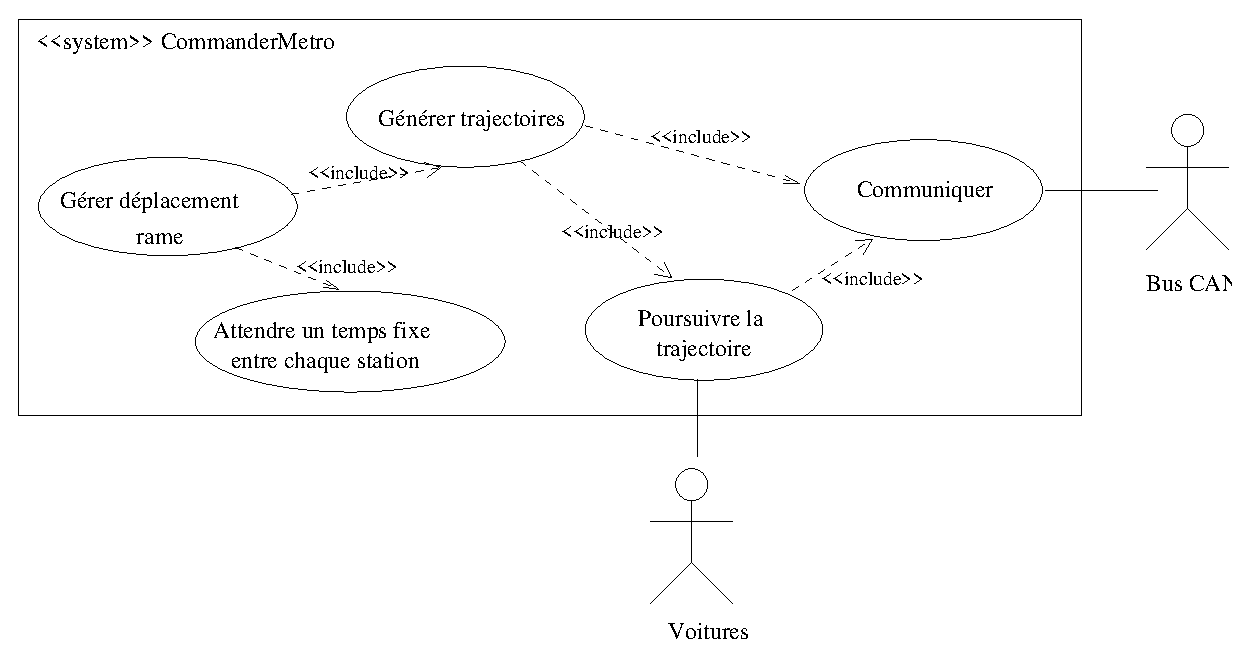
\includegraphics{useCase}}
  \end{center}
  \caption{Cas d'utilisation}
  \label{FigUseCase}
\end{figure}



La fig. \ref{FigArchi} repr�sente l'architecture du
prototype montrant l'emplacement des diff�rents calculateurs
sur les voitures. Chaque voiture poss�de sont calculateur
C167 (carte MCB167NET) qui est reli� aux autres par un bus
CAN commun (c�bles s�rie sur les connecteur CAN des cartes
MCB167NET). Une calculateur suppl�mentaire est reli�e au bus
CAN afin d'accueillir le g�n�rateur de trajectoires et le
point d'acc�s de d�bogage.

\begin{figure*}[bthp]
  \begin{center}
    \resizebox{0.85\linewidth}{!}{\inputxfig{./figures/archi2}}
  \end{center}
  \caption{Architecture du projet}
  \label{FigArchi}
\end{figure*}




Plusieurs projets ont d�j� �t� men�s � terme~:
\begin{itemize}
\item la conception m�canique des prototypes~;
\item la cha�ne d'acquisition de position et de vitesse
  ainsi que la commande de puissance du moteur~;
\item les \emph{driveurs} logiciels du moteur et des
  capteurs~;
\item la mod�lisation et l'identification du syst�me d'une
  voiture~;
\item un outil de transfert de donn�es entre le C167 et
  Matlab pour le d�bugage.
\end{itemize}

\label{SSecVusSys}

Le sch�ma technique de la figure~\ref{FigRameEtMicro}
concerne uniquement une voiture de la rame. 

\begin{figure*}[h!t]
  \begin{center}
    \resizebox{0.7\linewidth}{!}{\inputxfig{./figures/schema_technique}}
    \caption{Sch�ma technique de la maquette (trottinette)
      d'une voiture de la rame}
    \label{FigRameEtMicro}
  \end{center}
\end{figure*}


\section{Actionneur} 
De mani�re tr�s similaire � une v�ritable voiture de m�tro,
le moteur est command� par une premi�re boucle de r�gulation de
courant (permettant de le limiter). Le C167 en fonction de
ses mesures envoie la consigne de courant de mani�re �
asservir la position ou la vitesse de la voiture.

Le C167 envoie une consigne de courant au format PWM � la
carte de r�gulation de courant~:
\begin{itemize}
\item un rapport cyclique de 0\% correspond � un courant
  n�gatif maximal (-10A)~;
\item un rapport cyclique de 100\% correspond � un courant
  maximal de 10A~;
\item un rapport cyclique de 50\% commande un courant nul.
\end{itemize}

\section{Capteurs}
    
\begin{description}
\item [Vitesse] -- une g�n�ratrice tachym�trique permet de
  mesurer la vitesse de rotation du moteur et donc la
  vitesse de la voiture. La tension de la g�n�ratrice varie
  entre +10V et -10V lorsque la vitesse varie entre +3,33
  m/s et -3,33 m/s. La carte d'interface permet de ramener
  cette gamme de tension entre 0 et 5 Volts pour �tre
  convertie par un ADC du C167.
\item[Position] -- la position est mesur�e � l'aide de
  codeurs incr�mentaux. Il s'agit de deux capteurs optiques
  fixes d�tectant la pr�sence de bandes blanches ou noires
  (stries) fix�es sur la roue. Ses deux capteurs fournissent
  deux signaux binaires, nomm�s canal A et canal B, de forme
  carr�e lorsque la roue tourne � vitesse constante. En
  d�calant la bande de stries du canal A par rapport au
  canal B on peut d�tecter le sens de rotation de la roue et
  donc compter ou d�compter le nombre d'impulsions re�ues
  sur les canaux. On obtient ainsi une mesure de la position
  de la roue relative � la position initiale.

  Les canaux A et B sont connect�s � l'unit�e CAPCOM du C167
  de mani�re � g�n�rer des interruptions � chaque changement
  d'�tat d'un canal.
\item [Consignes] -- la consigne de position/vitesse est
  re�ue sur le C167 par la liaison du bus CAN. Le bus CAN
  permet aussi d'acc�der aux mesures de position et vitesse
  des autres voitures de mani�re � �viter les collisions.
\end{description}




\section{Librairie de p�riph�riques}
\label{SSecGestionnairePeriph}
\label{PartPeriphs}


Une librairie vous est livr�e \og clef en main \fg{}
\texttt{driveurs\_2008a.c} et \texttt{driveurs\_2008a.h} qui permet de
g�rer ces p�riph�riques\footnote{Merci � Thierry Rocacher
  pour ces biblioth�ques de p�riph�riques}. Le fichier
d'ent�te contient toutes les informations quand �
l'utilisation de cette librairie dont voici les fonctions
principales.

\subsection{Acquisition de la position -- TIMER 3 --}
Le timer 3 en mode \textit{incremental interface mode} permet de mesurer la position angulaire relative d'une roues.

Les fonctions associ�es sont~:
\begin{description}
\item[void Init\_Position(int Position)] initialise la
  position relative mesur�e en nombre de pas (largeur d'un
  strie du codeur incr�mental de 4,254 mm environ ;-)~;
\item[int Lire\_Position(void)] donne la position
  relative en nombre de pas.
\end{description}

\subsection{Acquisition de la vitesse -- ADC --}
L'unit� charg�e d'acqu�rir la vitesse consiste � lancer la
conversion analogique num�rique lorsque une demande de
mesure est effectu�e

Les fonctions associ�es sont~:
\begin{description}
\item[signed int Lire\_Vitesse()] renvoie un entier sign�
  entre -512 et +511 proportionnel � la vitesse.
\item[float Lire\_Vitesse\_float()] renvoie un flottant
  entre -3.3 et +3.3 qui repr�sente la vitesse en
  m.s\up{-1}.
\end{description}
       
\subsection{Commande du courant -- PWM --}
La consigne de courant envoy�e au r�gulateur de courant est
un signal PWM.

Les fonctions associ�es sont~:
\begin{description}
\item[void Fixe\_Rapport(float Commande\_Courant)] fixe le
  rapport cyclique de l'unit� PWM � la valeur\\
  \texttt{Commande\_Courant} au format flottant $\in
  [-1.0;+1.0]$~; l'annulation du courant peut �tre effectu�e
  par l'appel de la fonction \texttt{Fixe\_Rapport(0.0)}.
\end{description}



\chapter{Cahier des charges}

Vos travaux concerneront uniquement le prototype miniature
de la rame de m�tro d�nomm� dans la suite
\emph{m�trottinette}.
Vous vous engagez �~:
\begin{itemize}
\item \S \ref{PartCan} -- d�velopper la librairie de communication sur le bus
  CAN~;
\item \S \ref{PartTraject} -- d�terminer les param�tres de la trajectoire du m�tro
  entre deux stations~;
\item \S \ref{PartAutom} -- d�velopper un simulateur
  (Matlab/Simulink) de la rame compl�te et d�terminer un retour
  d'�tat global permettant de suivre une trajectoire donn�e
  sans collision~;
\item \S \ref{PartInfo} -- sp�cifier/d�velopper/tester le
  logiciel g�n�rique embarqu� sur chaque voiture, ainsi que
  le logiciel sp�cifique au g�n�rateur de trajectoires
  incluant une liaison de d�boguage avec matlab.
\end{itemize}


\section{Architecture logicielle}
Au cours de ce bureau d'�tude, la rame sera compos�e de
trois voitures. Vous devrez cependant prendre en compte le
fait que ce nombre pourra �tre modifi�. Pour cela la clef
\texttt{NB\_VOITURES = n} doit �tre d�finie pour indiquer le
nombre \emph{n} de voitures dans la rame.

Le logiciel final sera un projet Keil incluant les fichiers
et les librairies. Ce projet permettra de compiler et
d'ex�cuter n'importe quelle cible en d�finissant uniquement
la valeur de la clef de compilation qui lui correspond~:
\begin{itemize}
\item \texttt{ID\_VOITURE = x} indique qu'il faut g�n�rer le
  logiciel embarqu� sur la voiture num�ro $x \in 1..n$~;
\item \texttt{CONTROLEUR} indique qu'il faut g�n�rer le code
  du g�n�rateur de trajectoire/d�bogueur. 
\end{itemize}

Les clefs de compilation seront d�finies dans la partie
\emph{define} de l'onglet \textbf{C166} de configuration du
compilateur.



\section{Profil de trajectoire}
\label{PartTraject}
Le g�n�rateur de trajectoires donne les consignes de vitesse
$v_c(t)$ et de position $x_c(t)$, �videmment l'une est la
d�riv�e de l'autre $v(t)=\dot{x}(t)$.

La trajectoire d�butant � l'instant $t_0$ et se terminant �
l'instant $t_F$ doit respecter les contraintes suivante~:
\begin{itemize}
\item la position finale $x(t_F)$ doit se trouver � une
  distance $L$ de la position initiale $x(t_0)$
  correspondant � la distance entre chaque station de m�tro~;
\item la vitesse de la rame doit �tre limit�e �
  $V_{max}=3.33 \,\, m/s$~;
\item l'acc�l�ration de la rame ne doit jamais d�passer en
  valeur absolue l'acc�l�ration maximale
  $\left|\dot{v}(t)\right|<\gamma_{max}$
\end{itemize}

\begin{figure*}[h!tb]
  \centering
  \resizebox{0.72\linewidth}{!}{\inputxfig{./figures/profil}}
  \caption{Profil d'une trajectoire de consigne}
  \label{FigProfil}
\end{figure*}

La figure~\ref{FigProfil} montre le profil d'acc�l�ration,
le profil de vitesse et de position qui en d�coulent. La
trajectoire est g�n�r�e � partir d'un profil d'acc�l�ration
en trois phases~: acc�l�ration de dur�e $T_a=2s$, vitesse
constante de croisi�re, d�c�l�ration de dur�e $T_d=Ta=2s$.

Pour chaque voyage vers une station de m�tro situ�e � une
distance $L$, le g�n�rateur de trajectoire doit planifier le
profil de trajectoire adapt� et envoyer p�riodiquement les
consignes (toutes les 20 ms).

\subsection{D�livrables}
Calculez les expressions analytiques des param�tres du
profil de trajectoire de la figure~\ref{FigProfil}
connaissant la distance $L$ � parcourir, la vitesse de
croisi�re $V_{max}$, et les temps
d'acc�l�ration/d�c�l�ration $T_a=T_d$
% -----------------------------------------------------------------------
% \resizebox{!}
\begin{figure*}[h!t]
  \begin{center}
    \centering \resizebox{0.8\linewidth}{!}{\inputxfig{./figures/rampe}}
  \end{center}
  \caption{Le profil de trajectoire discr�tis�}
  \label{FigRampe}
\end{figure*}
% -----------------------------------------------------------------------

Ce calcul devra �tre r�alis� en temps discret (p�riode de
$T_c = 20ms$) par le calculateur comme l'indique la
fig.~\ref{FigRampe}.
\important{ Vous devrez fournir un fichier
\emph{simulink} mod�lisant le calcul en temps discret du
profil de trajectoire.
}


\cleardoublepage
\chapter {Mod�le d'une voiture}
\label{PartModeleAutom}
La commande de puissance du moteur est r�alis�e par une
structure en cascade � double boucle~:
\begin{itemize}
\item une premi�re boucle actionne le hacheur de mani�re �
  asservir le courant dans l'induit du moteur, sa dynamique
  est rapide puisque li�e aux constantes de temps
  �lectriques du moteur~;
\hyphenation{con-si-gne}
\item une deuxi�me boucle commande le courant de consigne de
  la premi�re de mani�re � asservir la trajectoire de la
  voiture, sa dynamique est plus lente car li�e aux
  constantes de temps m�canique de la voiture. 
\end{itemize}

La boucle de courant est d�j� assur�e par un r�gulateur PI
analogique (carte courant). La derni�re boucle est �
concevoir par vos soins et sera implant�e de mani�re
num�rique dans le C167.

Cette structure de boucle en cascade est tr�s utilis�e en
commande de puissance puisqu'elle permet de limiter le
courant d'induit en limitant l'amplitude de la consigne de
courant. Dans notre cas le courant est limit� � $\pm 10A$.  

Nous cherchons � mod�liser le syst�me \og vu par le
micro--contr�leur \fg{} comme repr�sent� dans la
fig.~\ref{FigMECA}.

\begin{figure*}[htbp]
  \centering
  \inputxfig{./figures/bloc_meca}
  \caption{Mod�le d'une voiture dans la bande 0--300Hz
    ($K_{PWM}=5V$, $S_I\approx 0,55\,\,\,A/V$,
    $\frac{K_\Phi}{J_v}\approx 22\,\,\, m/A/s^{2}$,
    $K_{tach}=\frac{2,5}{3,33}\,\,\, V.s/m$, $\Delta=
    4,254\,\,\, mm$)}
  \label{FigMECA}
\end{figure*}

\section{Identification}

Une s�rie d'�chelon de commande de courant a �t� envoy�e et les mesures de vitesse (avec \textit{signed int lire\_vitesse()}) et de position (avec \textit{int lire\_position()}) ont �t� enregistr�e sur le C167 puis renvoy�es vers Matlab.

Une premi�re identification donne la fonction de transfert en vitesse entre la commande de rapport cyclique $\sigma \in [-1 \quad 1]$ et la vitesse mesur�e $v \in [-512 \quad 511]$ suivante :
\begin{eqnarray}
	G(p) = \frac{v(p)}{\sigma(p)}= \frac{K}{1 + \tau p}\\
	K = 485 \mbox{ � } 10\% \nonumber \\
	\tau = 40 \mbox{ � } 100 \mbox{ ms} \nonumber
\end{eqnarray}

Le gain et la constante de temps peuvent varier � cause de l'incertitude due � la charge d'inetrie : rame vide ou rame pleine d'usager.

Une deuxi�me identification permet d'obtenir le gain d'int�gration entre la vitesse mesur�e $v$ et la position mesur�e $x$~:
\begin{eqnarray}
\frac{x(p)}{v(p)}=\frac{K_D}{p}\\
K_D = 1.919 \nonumber
\end{eqnarray}
Cette valeur est tr�s pr�cise car elle d�pend uniquement de la sensibilit� des capteurs.

\section{Mod�le d'�tat}

Dans la suite nous allons mod�liser l'ensemble des voitures
d'une rame. De mani�re � traiter ce probl�me de commande
multivariable il faut �crire le mod�le dans l'espace d'�tat.

On peut ainsi repr�senter le syst�me de la i\up{�me} voiture
d'une rame par l'�quation d'�tat~:
\begin{equation}
  \label{eq:etat}
  \left\{
    \begin{array}[l]{l}
      \dot{X_i} = A_i\,X_i + B_i\,u_i + G_i\,w_i\\
      Y_i = C_i\, X_i
    \end{array}
  \right.
\end{equation}

Dans ce cas l'entr�e $u_i$ du syst�me est la commande de
courant $\sigma$, l'entr�e de perturbation $w_i$ est le
courant $I_{per}$ �quivalent � la perturbation
$\Gamma_{per}$. Le vecteur d'�tat sera
$X_i(t)=\left[v(t)\quad x(t)\right]^T$, et la sortie sera
$Y=\left[vitesse(t) \quad position(t)\right]^T$


Ainsi on peut facilement repr�senter le mod�le d'une rame de
m�tro compos�e de N voitures en concat�nant les mod�les avec
une repr�sentation d'�tat \og augment�e\fg{}~:
\begin{equation}
  \label{eq:etat}
  \left\{
    \begin{array}[l]{llll}
      &\,\matNM{2N}{2N}\quad |_{_{2N}} 
      & \matNM{2N}{N} |_{_{N}}  & \matNM{2N}{N} |_{_{N}}\\
      \dot{X} &= A\qquad X  &+ B\qquad U &+ G\qquad W\\
      &\,\matNM{2N}{2N}\quad |_{_{2N}} & &\\
      Y &= C\qquad X & &\\
    \end{array}
  \right.
\end{equation}

Le vecteur d'�tat est augment� et devient $X=\left[ X_1
  \ldots X_N\right]^T$, le vecteur des entr�es devient
$U=\left[ u_1 \ldots u_N \right]^T$, celui des perturbations
$W=\left[ w_1 \ldots w_N \right]^T$ et le vecteur des
sorties sera $Y=\left[Y_1 \ldots Y_N \right]^T$.

Il est alors possible d'appliquer des m�thodes de conception
dans l'espaces d'�tat � ce syst�me multivariable (retour
d'�tat, observateurs, commande optimale).



\end{document}

